\documentclass[14pt]{beamer}
\setbeamertemplate{itemize item}{$\bullet$}
\setbeamertemplate{navigation symbols}{}
\setbeamertemplate{mini frames}{}
\setbeamertemplate{section in toc}[sections numbered]
\setbeamertemplate{itemize items}[square]
\setbeamercolor*{item}{fg=gray}
\usecolortheme{dove}
\hypersetup{pdfpagemode=FullScreen}

\usepackage[yyyymmdd]{datetime}

% Define some accent colors:
\definecolor{DarkFern}{HTML}{407428}
\definecolor{DarkCharcoal}{HTML}{4D4944}
\colorlet{Fern}{DarkFern!85!white}
\colorlet{Charcoal}{DarkCharcoal!85!white}
\colorlet{LightCharcoal}{Charcoal!50!white}
\colorlet{AlertColor}{orange!80!black}
\colorlet{DarkRed}{red!70!black}
\colorlet{DarkBlue}{blue!70!black}
\colorlet{DarkGreen}{green!70!black}
\definecolor{palecerulean}{rgb}{0.61, 0.77, 0.89}

% Use the colors:
\setbeamercolor{alerted text}{fg=palecerulean}
\setbeamercolor{title}{fg=blact}

% Create horizontal rule, header, and title page
\makeatletter
\def\vhrulefill#1{\leavevmode\leaders\hrule\@height#1\hfill \kern\z@}
\makeatother
\setbeamertemplate{frametitle}{\color{black}\bfseries\insertframetitle\par\vskip-6pt\color{palecerulean}\vhrulefill{1.75pt}}
\defbeamertemplate*{title page}{customized}[1][]
{
	{\begin{centering}
	\usebeamerfont{title}\bfseries\inserttitle\par\bigskip
	\usebeamerfont{subtitle}\insertsubtitle\par\vskip-3pt\color{palecerulean}\vhrulefill{1.75pt}\color{black}\\
	\bigskip
	\bigskip
	\usebeamerfont{author}\insertauthor\par\bigskip
	\usebeamerfont{institute}\insertinstitute\par
	\usebeamerfont{date}\insertdate\par
	\usebeamercolor[fg]{titlegraphic}\inserttitlegraphic
				\insertframetitle\par
	\smallskip\end{centering}}
}


\title{My Presentation}
\subtitle{Using Beamer}
\author{Anthony Kevins}
\institute{School of Governance\\
	Utrecht University}
\date{\today}


\begin{document}

\begin{frame}
\titlepage
\end{frame}

\begin{frame}
\frametitle{Table of Contents}

\tableofcontents
\end{frame}


\section{Getting Started}

\begin{frame}
\frametitle{Title}
Lorem ipsum dolor sit amet, consectetur adipisicing elit, sed do eiusmod tempor incididunt ut labore et dolore magna aliqua.
\end{frame}


\section{Lists etc.}
\begin{frame}
	\frametitle{Research Design}
	\begin{itemize}[<+-| alert@+>]
		\item<1-> \alert<+>{DV:} Perceived impact of immigrants on the economy
		\item<2-> \alert<+>{Key variables:} outsiderness scores, independently and interacted with GDP (PPP) and national unemployment rates
		\item<3-> \alert<+>{Key individual-level controls:} factors related to precarity (e.g. education, union membership, labour market status, income decile)
		\item<4-> \alert<+>{Key country-level controls:} changes in GDP, \% of foreign-born population, and \% of migrant population with tertiary education
		\item<5-> \alert<+>{Models:} GLS with country fixed effects and MLE with design and population weights
	\end{itemize}
\end{frame}

\begin{frame}
\frametitle{List}
\begin{enumerate}[I]
	\item Point A
	\item Point B
	\begin{enumerate}[i]
		\item part 1
		\item part 2
	\end{enumerate}
	\item Point C
	\item Point D
\end{enumerate}
\end{frame}


\begin{frame}
\frametitle{Using Columns}
\begin{columns}
	\column{0.5\textwidth}
	Lorem ipsum dolor sit amet, consectetur adipisicing elit, sed do eiusmod tempor incididunt ut labore et dolore magna aliqua.
	\column{0.5\textwidth}
	Lorem ipsum dolor sit amet, consectetur adipisicing elit, sed do eiusmod tempor incididunt ut labore et dolore magna aliqua.
\end{columns}
\end{frame}

\begin{frame}
\frametitle{Pictures}
\begin{figure}
	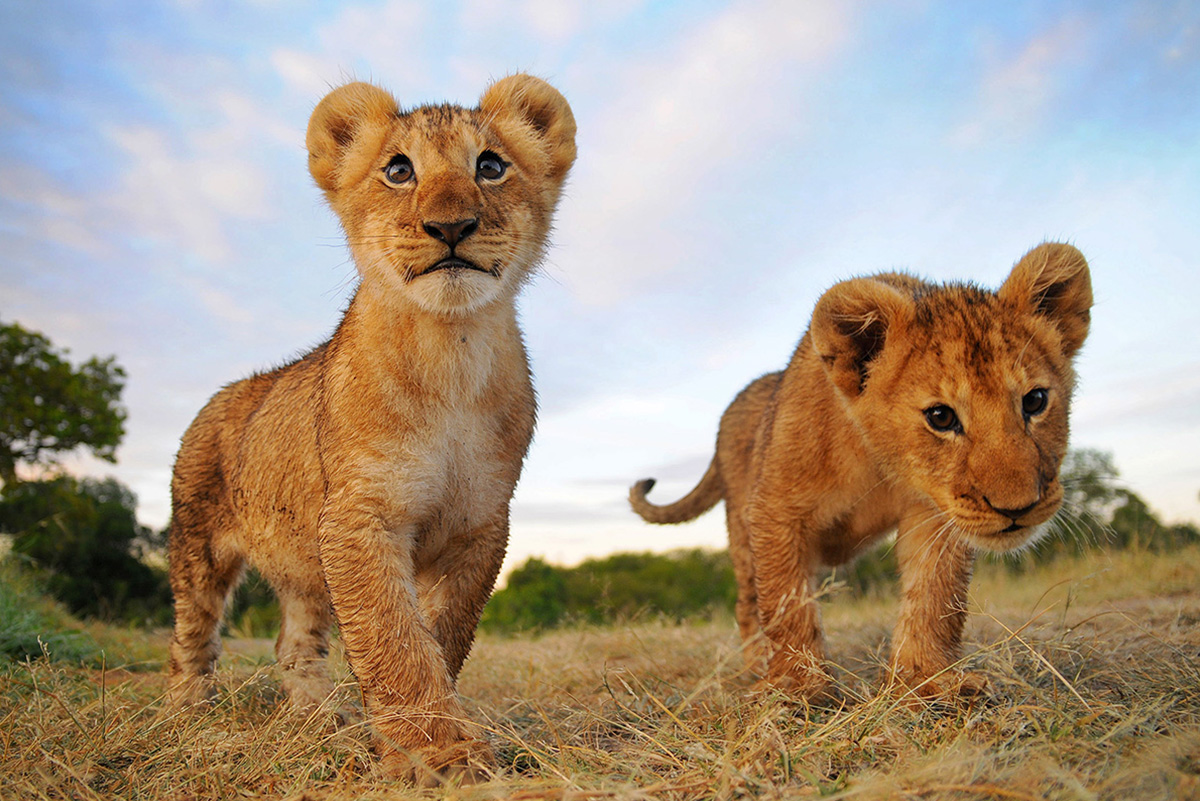
\includegraphics[width=\textwidth]{Lion}
	\caption{lions!!}
\end{figure}
	Lorem ipsum dolor sit amet, consectetur adipisicing elit, sed do eiusmod tempor incididunt ut labore et dolore magna aliqua.
\end{frame}

\begin{frame}
\begin{table}
	\begin{tabular}{l | c | c | c | c }
		Competitor Name & Swim & Cycle & Run & Total \\
		\hline \hline
		John T & 13:04 & 24:15 & 18:34 & 55:53 \\
		Norman P & 8:00 & 22:45 & 23:02 & 53:47\\
		Alex K & 14:00 & 28:00 & n/a & n/a\\
		Sarah H & 9:22 & 21:10 & 24:03 & 54:35
	\end{tabular}
	\caption{Triathlon results}
\end{table}
\end{frame}


\section{Blocks etc.}

\begin{frame}
\begin{block}{Block Title}
	Lorem ipsum dolor sit amet, consectetur adipisicing elit, sed do eiusmod tempor incididunt ut labore et dolore magna aliqua.
\end{block}

\begin{alertblock}{Block Title}
	Lorem ipsum dolor sit amet, consectetur adipisicing elit, sed do eiusmod tempor incididunt ut labore et dolore magna aliqua.
\end{alertblock}

\begin{definition}
	A prime number is a number that...
\end{definition}

\begin{example}
	Lorem ipsum dolor sit amet, consectetur adipisicing elit, sed do eiusmod tempor incididunt ut labore et dolore magna aliqua.
\end{example}
\end{frame}


\begin{frame}
\label{contents}
\hyperlink{contents}{click here}

\hyperlink{contents}{\beamerbutton{contents page}}

Here are some other button commands we can use.

\hyperlink{columns}{\beamergotobutton{columns page}}

\hyperlink{pictures}{\beamerskipbutton{pictures page}}

\hyperlink{pictures}{\beamerreturnbutton{pictures page}}


\end{frame}


\section{Overlay Specifications}

\begin{frame}
\frametitle{List}
\begin{itemize}
	\pause
	\item Point A
	\pause
	\item Point B
	\begin{itemize}
		\pause
		\item part 1
		\pause
		\item part 2
	\end{itemize}
	\pause
	\item Point C
	\pause
	\item Point D
\end{itemize}
\end{frame}

\begin{frame}
\frametitle{More Lists}
\begin{enumerate}[(I)]
	\item<1-> Point A
	\item<2-> Point B
	\begin{itemize}
		\item<3-> part 1
		\item<4-> part 2
	\end{itemize}
	\item<5-> Point C
	\item<6-> Point D
\end{enumerate}
\end{frame}

\begin{frame}
\frametitle{Overlays - Simple}

\onslide<1->{First Line of Text}

\onslide<2->{Second Line of Text}

\onslide<3->{Third Line of Text}
\end{frame}

\begin{frame}
\frametitle{Overlays - Transparent}

\setbeamercovered{transparent}
\onslide<1->{First Line of Text}

\onslide<2->{Second Line of Text}

\onslide<3->{Third Line of Text}
\end{frame}

\begin{frame}
\frametitle{Overlays - Only}
\only<1>{First Line of Text}

\only<2>{Second Line of Text}

\only<3>{Third Line of Text}
\end{frame}

\begin{frame}
\textbf<2>{Example Text}

\textit<2>{Example Text}

\textsl<2>{Example Text}

\textrm<2>{Example Text}

\textsf<2>{Example Text}

\textcolor<2>{orange}{Example Text}

\alert<2>{Example Text}

\structure<2>{Example Text}
\end{frame}


\setbeamercovered{invisible}
\begin{frame}
\frametitle{Tables}
\begin{table}
	\begin{tabular}{l | c | c | c | c }
		Competitor Name & Swim & Cycle & Run & Total \\
		\hline \hline
		John T & 13:04 & 24:15 & 18:34 & 55:53 \onslide<2-> \\
		Norman P & 8:00 & 22:45 & 23:02 & 53:47 \onslide<3->\\
		Alex K & 14:00 & 28:00 & n/a & n/a \onslide<4->\\
		Sarah H & 9:22 & 21:10 & 24:03 & 54:35
	\end{tabular}
	\caption{Triathlon results}
\end{table}
\end{frame}


\section{Themes and Handouts}

\begin{frame}[fragile]
\frametitle{To make a handout}
\begin{semiverbatim}
	\\documentclass[handout]{beamer}
	\\usepackage{pgfpages}
	\\pgfpagesuselayout{2 on 1}[a4paper,border shrink=5mm]
\end{semiverbatim}
\end{frame}

\end{document}
